\documentclass[12pt]{article}
\usepackage[margin=2cm]{geometry}
\usepackage{amsmath,amssymb,amsthm}
\usepackage{graphicx}
% For subfigure environments
\usepackage{subcaption}
\usepackage[framemethod=tikz]{mdframed}

% Optional: for [H] specifier
\usepackage{float}

\graphicspath{ {./images/} }


\title{\vspace{2cm}
    \Huge \textbf{Heuristic Optimization Techniques}\\[2cm]
    \LARGE Report 1
    \vspace{10cm}
    
    \large Aksinia Vorobeva, 12044614  \\ Marcel Korinek, 12220824
    }

\begin{document}

\maketitle


\pagebreak

\section{Problem Description}
\begin{mdframed}[
    linecolor=black,
    linewidth=1.5pt,
    roundcorner=5pt,
    backgroundcolor=blue!5,
    userdefinedwidth=\textwidth,
]
\textbf{Selective Capacitated Fair Pickup and Delivery Problem (SCF-PDP)}

\vspace{0.7em}
\textbf{Graph model:}  
Complete directed graph $G = (V, A)$, where:
\begin{itemize}
    \item $V$ contains the depot as well as all pickup and drop-off locations.
    \item $A = \{(u,v) : u, v \in V, u \neq v\}$ represents travel arcs.
    \item Each arc $(u,v)$ has an associated distance  
    \[
        a_{u,v} = \left\lceil \sqrt{(x_u - x_v)^2 + (y_u - y_v)^2} \right\rceil,
    \]
    where $(x_u, y_u)$ are the coordinates of location $u$.
\end{itemize}

\vspace{0.5em}
\textbf{n Customer requests:}   
For each request $i \in \{1, \dots, n\}$ there are:
\[
v_i^{\uparrow} \in V \quad \text{(pickup location)}, \qquad
v_i^{\downarrow} \in V \quad \text{(drop-off location)}.
\]

The solution must serve at least $\gamma \le n$ of them.

\vspace{0.5em}
\textbf{Vehicles:}  
A fleet $K$ of $n_K$ identical vehicles is available, each with capacity $C$ and starting/ending at the depot.

\vspace{0.7em}
\textbf{Feasible solution:}  
A solution consists of a route $R_k$ for each vehicle $k \in K$, where $R_{k,i}$ denotes the $i$-th stop. Each solution must satisfy:
\begin{itemize}
    \item Vehicle load never exceeds capacity $C$
    \item Each served request is fully handled by a single vehicle
    \item At least $\gamma$ requests are served in total
\end{itemize}

The travel duration of route $R_k$ is
\[
d(R_k)
= a_{\text{depot}, R_{k,1}}
+ a_{R_{k,|R_k|}, \text{depot}}
+ \sum_{(u,v)\in R_k} a_{u,v}.
\]

\vspace{0.5em}
\textbf{Fairness measure:}  
We use the Jain fairness index:
\[
J(R)
=
\frac{\left(\sum_{k \in K} d(R_k)\right)^2}
{\,n_K \cdot \sum_{k \in K} d(R_k)^2\, }.
\]

\vspace{0.7em}
\textbf{Objective:}  
Minimize the total travel duration penalized by unfairness:
\[
\sum_{k \in K} d(R_k)
\;+\;
\rho \cdot (1 - J(R)),
\]
where $\rho$ controls the trade-off between efficiency and fairness.

\end{mdframed}

\subsection{Experimental Setup}

All experiments were made on a machine with a AMD Ryzen 7 9800X3D and 32 RAM, running Windows 11 and Python 3.13.9.

We tested every algortihm on all of the instances with size 50 and 100. For every non-deterministic algorithm we made at least three runs in order to increase the significance of the results.

For each experiment, the relevant algorithm configurations are provided in the corresponding chapter.

\section{Description of Algorithms}

Every algorithm shares five input parameters: \emph{customers}, \emph{vehicles}, \emph{to$\_$fulfilled}, \emph{rho} and \emph{output$\_$statistic}. 

\vspace{0.6em}
\textbf{Customers.}

The input parameter \emph{customers} is a list of \texttt{Customer} objects, each customer contains the relevant information for each request:

\begin{itemize}
    \item a unique identifier
    \item a pickup location and a drop-off location, both represented as \texttt{Point} objects
    \item the amount of goods to be transported
\end{itemize}

A \texttt{Point} object contains the coordinates, the point type (depot, pickup, drop-off),
and the quantity of goods associated with it (if the point type is pickup, then  the quantity of goods is positive for pickups, if it is drop-off, then the quantity is negative).

\vspace{0.6em}
\textbf{Vehicles.}

The most important parameter is \emph{vehicles}, which is also our choice of a solution representation for this problem. It is a list of \texttt{Vehicle} objects.
Each vehicle maintains the following:
\begin{itemize}
    \item its capacity
    \item its current load and position
    \item its route, stored as a sequence of \texttt{Point} objects
    \item its accumulated path length
    \item a load-history tracing the load after each visited point
\end{itemize}
Together, the set of vehicles encodes the full multi-vehicle our routing solution, including which requests are served and in what order.

\vspace{0.6em}
\textbf{Minimum Requests to Serve.}

The parameter \emph{to\_fulfill} describes the minimum number of requests to
be served.

\vspace{0.6em}
\textbf{Fairness Weight \boldmath$\rho$.}

The parameter \emph{rho} is the fairness weight in the objective function.
It is passed to the \texttt{ObjectiveTracker}, which evaluates
\[
\text{Objective}
=
\sum_{k} d(R_k)
\;+\;
\rho \cdot (1 - J(R)),
\]
and updates values efficiently using delta evaluation.

\vspace{0.6em}
\textbf{Output Statistics.}

The parameter \texttt{output\_statistic} is irrelevant for the functionality of the algorithms, as it is only relevant for the experimental evaluation and result analysis. We save the collection of detailed performance data using the \texttt{Statistic} class,
including:
\begin{itemize}
    \item the objective value over time
    \item fairness values over time
    \item total route duration over time
    \item the number of iterations performed
\end{itemize}

\vspace{1em}
\textbf{Algorithm output.}

Ultimately, at the end of the algorithm, we receive:

\begin{itemize}
    \item a file in .txt format with the final solution to the problem
    \item statistical data
    \item a graphical representation of the solution (see Figure~\ref{fig:graph_rep_sa})
\end{itemize}


\begin{figure}[H]
    \centering
    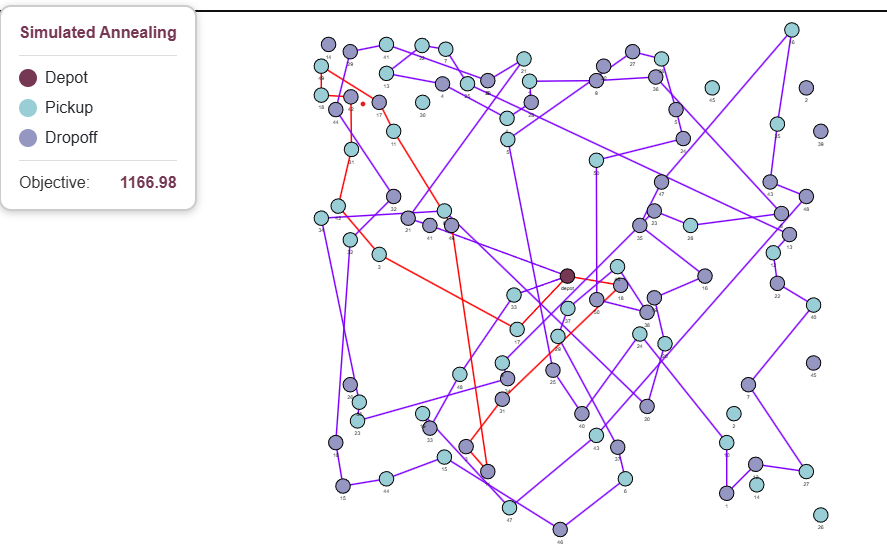
\includegraphics[width=\linewidth]{graphics/output_1.png}
    \caption{Graphical representation of SA output}
    \label{fig:graph_rep_sa}
\end{figure}

\subsection{Deterministic Construction Heuristic}

\subsubsection{The Basic Idea}

The first algorithm is a greedy variant of the Savings heuristic for the \textsc{(capacitated) vehicle routing problem (VRP)}. Our Deterministic Construction Heuristic is based on the modified Clarke-Wright Savings principle but contains a number of extensions:

\begin{itemize}
    \item Each customer is initially served by a separate temporary vehicle (one client per vehicle). The path is \[
        \text{depot} \rightarrow \text{pickup}_i \rightarrow \text{dropoff}_i \rightarrow \text{depot}.
    \]
    \item After that, for any two customers i and j, a savings value is computed by lazy evaluation as:
    \[
    S_{ij} = D(\text{depot}, i) + D(\text{depot}, j) - D(i, j),
\] 
where $D(a,b)$ — the distance between points $a$, $b$. At most the best $3$ $*$ \textbf{number of customers} results will be stored together with the corresponding customer pair in descending order in a \texttt{heapq}.
    \item The choice of a merger aims to minimize the objective function
    \item The process continues until the required number of clients served is reached
\end{itemize}

\vspace{0.6em}
\textbf{Attempt to merge paths.}

If customers $i$ and $j$ belong to different vehicles, then we merge the corresponding paths. We have implemented two different strategies for merging:

\paragraph{A. \texttt{merge\_without\_reordering} — pure construction.}

The paths are connected sequentially:
\[
    \text{Route A: depot} \rightarrow \dots \rightarrow \text{depot},
\]
\[
    \text{Route B: depot} \rightarrow \dots \rightarrow \text{depot},
\]
\[
    \text{Merged: depot} \rightarrow A \rightarrow B \rightarrow \text{depot}.
\]

\paragraph{B. \texttt{merge\_with\_reordering}.}

Pickups and dropoffs for two routes are combined into a single pool. A new route is constructed as follows:

\begin{enumerate}
\item Start at the depot.
\item At each step, select the closest available pickup that meets the load restrictions.
\item If there is no pickup that makes the solution feasible, then add the corresponding dropoff, thereby reducing the load.
\item After the pool is exhausted, a return to the depot is added.
\end{enumerate}

\vspace{0.6em}
\textbf{Evaluation of the quality of an intermediate solutions.}

After each potential merge, an updated list of routes is generated, where route $j$ is removed and route $i$ is replaced with the merged route. The objective function is then calculated:
\[
\text{objective} = \text{distance} + \rho \cdot (\text{number of vehicles}).
\]
Based on the results, the best merge will be selected for the current iteration.
The merging process stops if required number of clients is served.

\subsubsection{Comparison of Results}

From a comparison of the two strategies presented in Figure~\ref{fig:comparison_construction_1} we can see that the quality of the solution based on the objective value is much better by merging with reordering, but it needs more time to give a solution.

\begin{figure}[H]
    \centering
    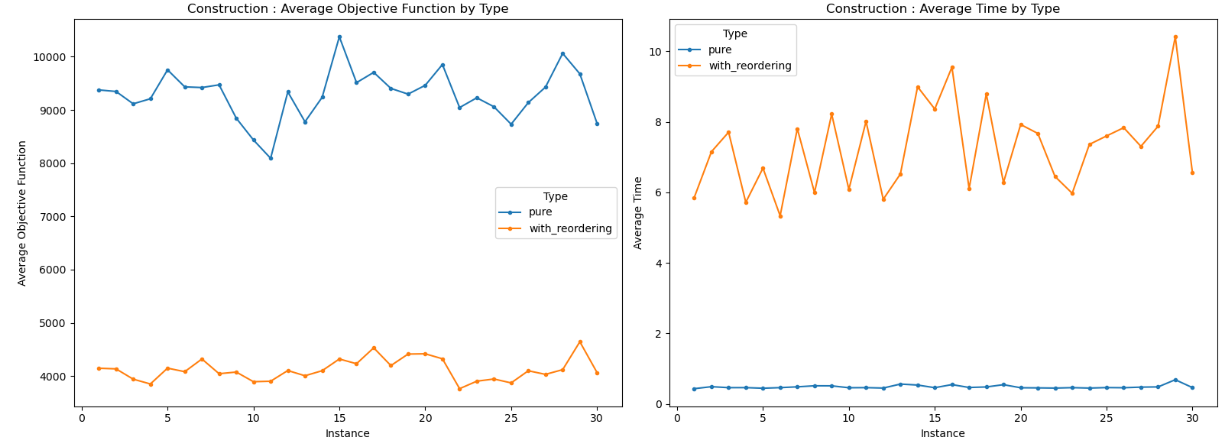
\includegraphics[width=\linewidth]{graphics/comparison_construction_1.png}
    \caption{Construction: Comparison of average Objective Function and Run Time for 100 customers}
    \label{fig:comparison_construction_1}
\end{figure}

The approach with reordering has the runtime:  \[
    O(L^2) \text{ for the reordering}, \quad O(N^2 L^2) \text{ in summary}.
\] while pure construction needs \[
    O(L) \text{ for one merge}, \quad O(L N^2) \text{ with considering of savings}.
\] (see Table~\ref{tab:c_str_prop})

\begin{table}[H]
    \centering
    \begin{tabular}{l|c|c}
        \textbf{Criterion} & \textbf{pure} & \textbf{with reordering} \\
        \hline
        The path quality & medium/low & high \\
        Speed &
        \( O(L),\; O(L N^2) \) &
        \( O(L^2),\; O(N^2 L^2) \) \\
        Sensitivity to order & high & low \\
    \end{tabular}
    \caption{Construction: Comparison of strategy properties}
\label{tab:c_str_prop}
\end{table}

And with the help of boxplots (see Figure~\ref{fig:comparison_construction_2}), it becomes clear how the number of clients affects runtime and objective value. As the number of clients increases, the time required to build a solution with construction heuristic using reordering increases significantly.

\begin{figure}[H]
    \centering
    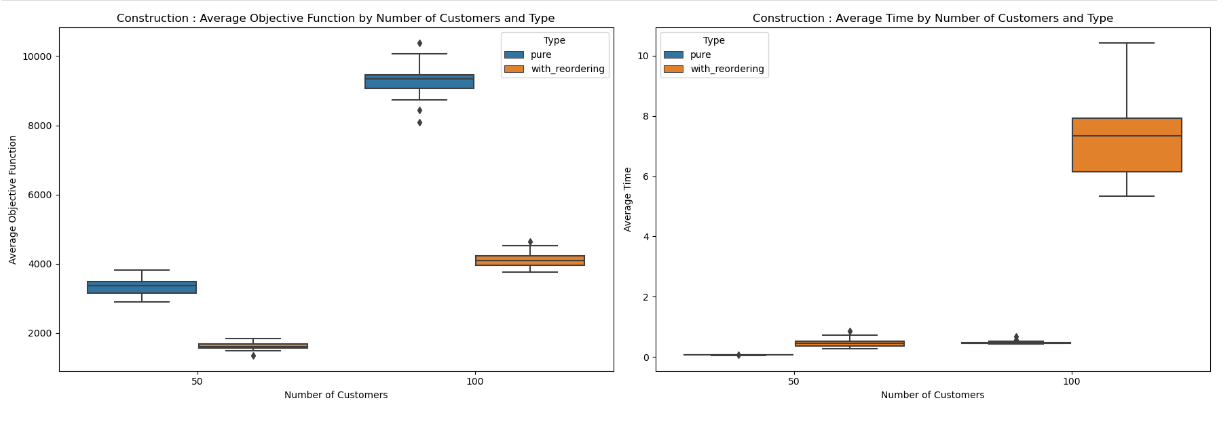
\includegraphics[width=\linewidth]{graphics/comparison_construction_2.png}
    \caption{Construction: Comparison of average Objective Function and Run Time Boxplots}
    \label{fig:comparison_construction_2}
\end{figure}

\subsection{Randomized Construction Heuristic}

The only difference to the deterministic construction heuristic is that instead of one best merged vehicle in each iteration, a restricted candidate list of merged vehicles is stored and one of them is chosen randomly. For this purpose, there exists another input parameter alpha, which defines how good the merged vehicles to be considered need to be at least. Its default is set to 0.3. A value of 1 would be completely random and a value of 0 would be the same as the deterministic construction.


\subsubsection{Comparison of Results}

Obviously, when comparing pure randomized construction and randomized construction with reordering, we will get the same distinctive features of each strategy as in deterministic construction heuristic. (see Figure~\ref{fig:comparison_construction_3} and Figure~\ref{fig:comparison_construction_4})

\begin{figure}[H]
    \centering
    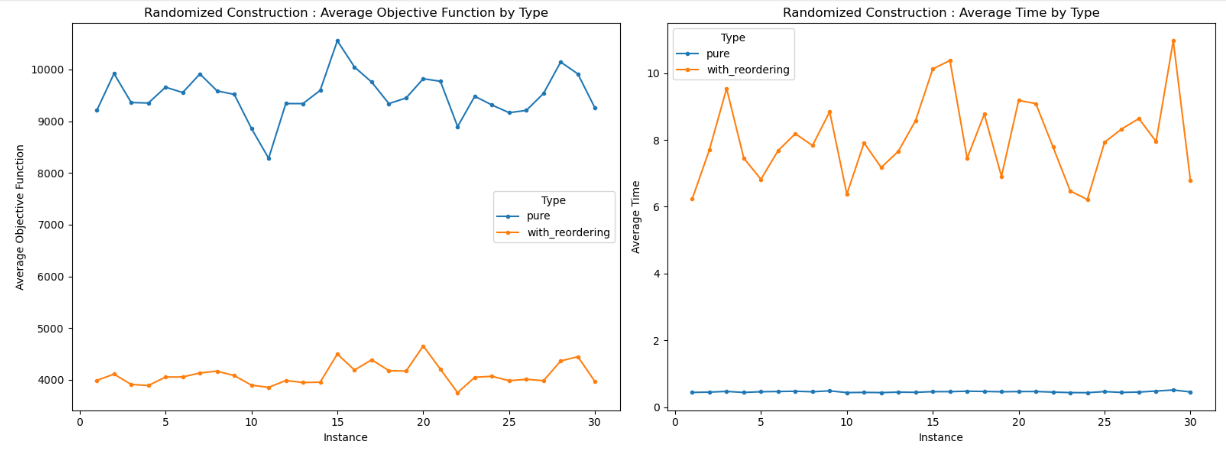
\includegraphics[width=\linewidth]{graphics/comparison_construction_3.png}
    \caption{Randomized Construction: Comparison of average Objective Function and Run Time for 100 customers}
    \label{fig:comparison_construction_3}
\end{figure}

\begin{figure}[H]
    \centering
    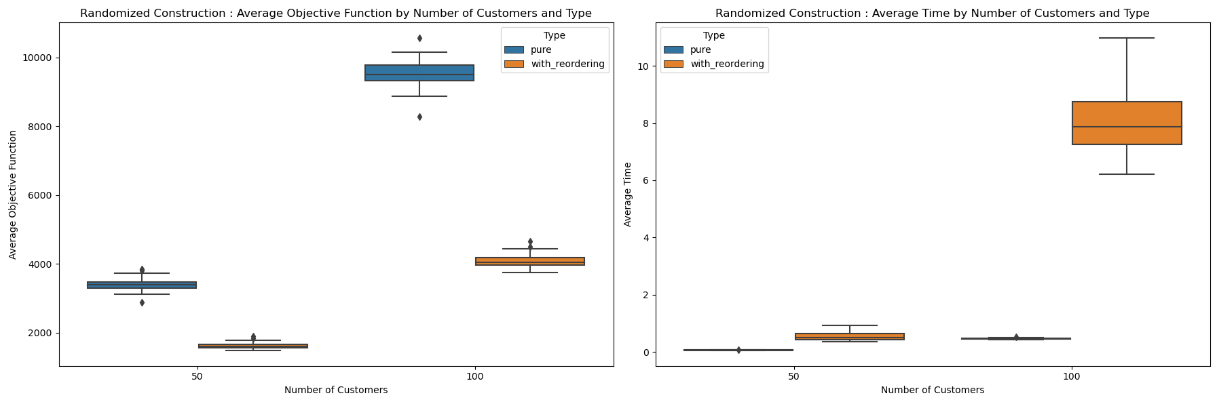
\includegraphics[width=\linewidth]{graphics/comparison_construction_4.png}
    \caption{Randomized Construction: Comparison of average Objective Function and Run Time Boxplots}
    \label{fig:comparison_construction_4}
\end{figure}

However, we wanted to know how the alpha parameter affects the quality of the solution. The Figure~\ref{fig:comparison_degree_rand}) does not give us much information about how the quality of the solution depends on the degree of randomization, but we can clearly see that the computation time increases slightly as alpha increases. It happens because with increasing alpha we become more candidate choices, requiring more processing time to evaluate them. In boxplot representation of results it becomes clear that the smaller alpha produces better objective values. 

\begin{figure}[H]
    \centering
    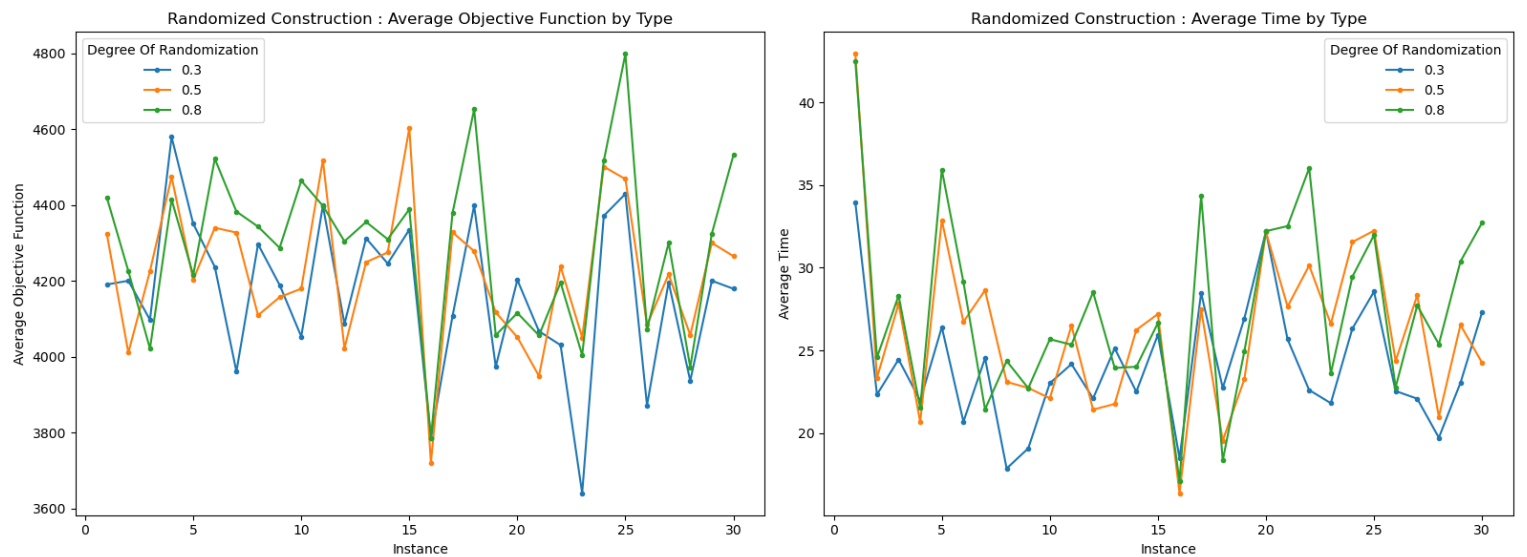
\includegraphics[width=\linewidth]{graphics/comparison_degree_rand.png}
    \caption{Randomized Construction: Impact of degree of randomization of average Objective Function and Run Time for 100 customers}
    \label{fig:comparison_degree_rand}
\end{figure}

\begin{figure}[H]
    \centering
    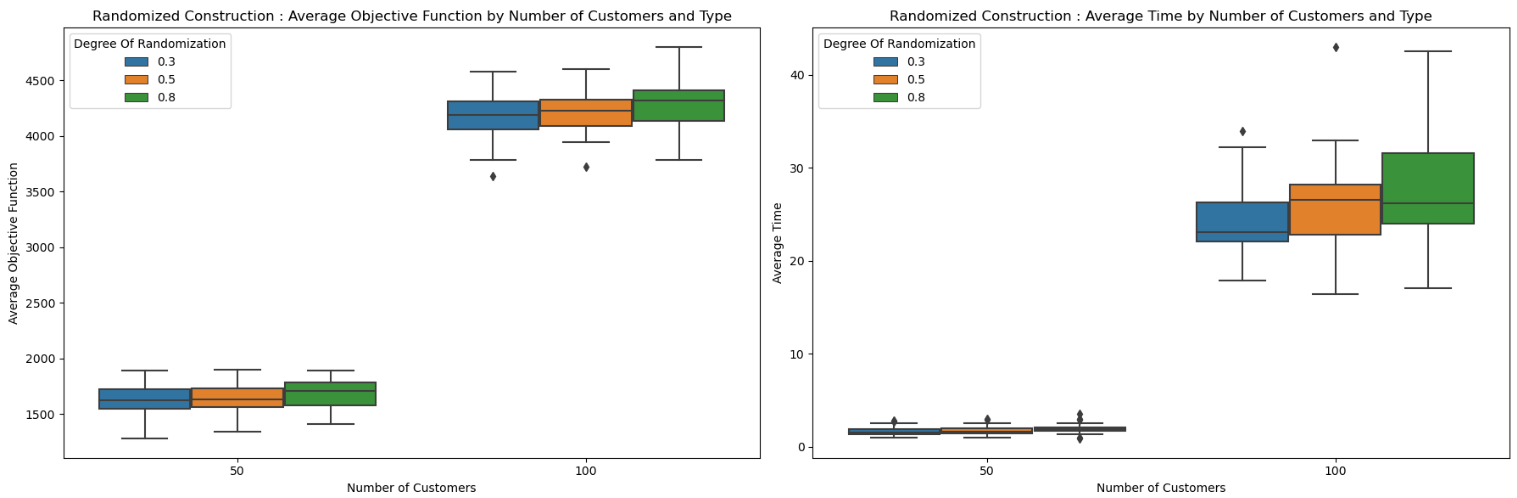
\includegraphics[width=\linewidth]{graphics/comparison_degree_rand_1.png}
    \caption{Randomized Construction: Impact of degree of randomization of average Objective Function and Run Time Boxplots}
    \label{fig:comparison_degree_rand_1}
\end{figure}

\subsection{Pilot Search}

The pilot search uses the pure deterministic construction heuristic in order to compare the quality of each incomplete solution per iteration.

The set of incomplete solutions of an iteration is constructed as follows. The first unfulfilled customer request in the list is treated as a short path (pickup, drop-off) which is inserted into each possible position right after the first depot point or right after another drop-off point. This ensures that the load is never exceeded and aligns perfectly with the construction heuristic, which also assigns pair-wise.

The pilot search performs at most $n$ iterations.  
In each iteration, the candidate set contains
\[
|C| = O(n_K \cdot n)
\]
because every unserved request can be inserted into each of the $n_K$ vehicles at $O(n)$ admissible positions.

For every candidate $c \in C$, we either run the construction heuristic or reuse a cached result.  
The construction heuristic runs in $O(n_K n^{2})$ time.

Hence one iteration costs
\[
O(|C| \cdot n_K n^{2}) 
= O(n_K n \cdot n_K n^{2})
= O(n_K^2 \cdot n^{3}).
\]

Over $n$ iterations the total runtime is
\[
O(n_K^2 \cdot n^{4}).
\]


The results of how much the solution improved after applying Pilot Search to pure deterministic construction heuristic can be found in Figure~\ref{fig:comparison_ps_pre_c}.

\begin{figure}[H]
    \centering
    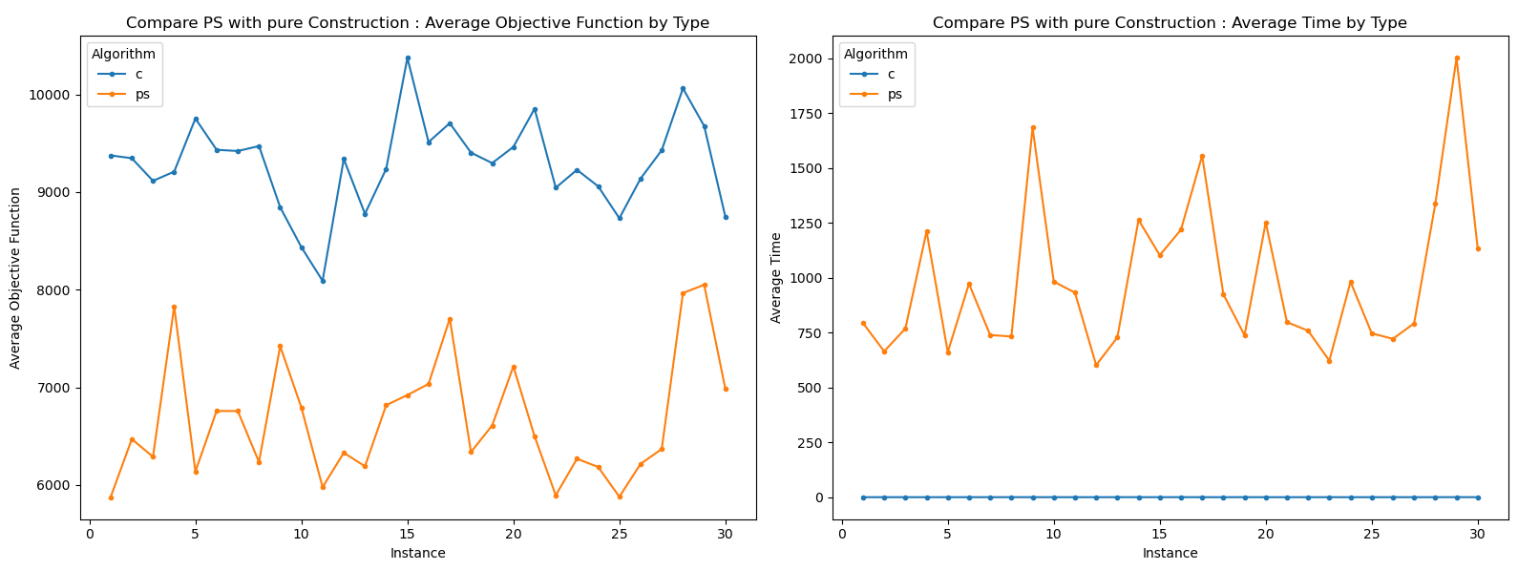
\includegraphics[width=\linewidth]{graphics/comparison_ps_pre_c.png}
    \caption{PS vs Pure Construction: Comparison of average Objective Function and Run Time for 100 customers}
    \label{fig:comparison_ps_pre_c}
\end{figure}

\subsection{Local Search}

The local search has the two additional input parameters \emph{neighborhood$\_$structure} and \emph{improvement$\_$strategy}. They control which neighborhood structure and which improvement strategy the local search should use.

The general implementation is very basic, the interesting parts lie within the neighborhood structures described in Section~\ref{neighborhood}.

\subsubsection{Neighborhood Structures}

We implemented five different neighborhood structures, which are described in the following paragraphs.

\label{neighborhood}

\paragraph{Exchange}

The exchange neighborhood was the first structure we implemented. As the name suggests, the current occurrences of pickup and drop-off points of two different customers are simply swapped. 

\bigskip

There are three different cases that need to be considered:

\medskip

If both customer requests are currently fulfilled by one vehicle, then the exchange happens only inside one vehicle.

\medskip

Another possible case is that one customer request is fulfilled by one and the other by another vehicle. In this case the exchange is happening between two different vehicles.

\medskip

In the third case one customer request is fulfilled by one vehicle and the other one is not yet fulfilled.

\bigskip

Independent of the case, the pickup point of the one customer is replaced by the pickup point of the other customer inside a vehicle path. The same holds for the corresponding drop-off points. The whole neighborhood consists of every possible swap and is therefore bounded in size by $O(\frac{n(n-1)}{2})$.

\paragraph{Pickup Relocate}

The pickup relocate neighborhood is even simpler than that. Here, a pickup point is relocated into every possible valid position of the same vehicle path. Relocations are only possible after the first depot point up until the corresponding drop-off point. With n customer requests in the worst case this yields approximately \textbf{n} $*$ \textbf{number of points in the corresponding vehicle path} different possibilities.

\paragraph{Dropoff Relocate}

This neighborhood is technically the same as the pickup relocate, only that instead of pickup points, drop-off points are relocated.

\paragraph{Remove and Append}

This neighborhood was a simple try to realize a move of customer requests to other vehicles. A pickup and drop-off point is removed from one vehicle path and appended to another vehicle path (right before the second depot point). The size of this neighborhood is at most n $*$ ($n_K$ - 1)

\paragraph{Move}

The move neighborhood is an improvement for the remove and append neighborhood, at cost of performance. Instead of simply appending both points to a path, all different possibilities to insert a pickup point and drop-off point into the path are considered. (a drop-off is not forced to be directly after the pickup point). This increases the size of the neighborhood to $n^3$ $*$ ($n_k$ - 1) (This is a loose upper bound)

\paragraph{Notes on Efficiency:}

The neighborhood structures were initially implemented as a full set of solutions, which means that for the best-improvement strategy we had to iterate over the whole set. Since this means that we would have to iterate two times over the set (since creating the set is also one full iteration), we decided to not return a set of all valid neighbors, but instead to choose only one neighbor depending on the strategy. This not only reduced the number of iterations by 1, but this also made the computation actually feasible, since in the initial idea for every neighbor a copy of the solution was created, which does not scale very well. Now, there is only one necessary deep copy for the neighbor we want to choose.

\medskip

In order to do this, we had to implement functions that compute (predict) the objective values of different neighbors without changing or duplicating the initial solution. In addition to that, we also used delta evaluation for the computation of the objective values by only updating necessary parts. We implemented this within the ObjectiveTracker object.
This allowed us to update the objective value in constant time instead of linear time, which would be needed in order to iterate over all vehicles (so instead of $O(n_K)$ we get $O(1)$).

\subsubsection{Comparison of Neighborhood Structures}

Figure~\ref{fig:comparison_ns_ls} and Figure~\ref{fig:comparison_ns_ls_1} show the comparison of objective values and runtimes of local search using these different neighborhood structures. Interestingly, the drop-off relocate neighborhood leads to the best results most of the time. The structure with the highest objective values is the move and append neighborhood, followed by the move neighborhood. Neighborhoods that apply changes within vehicles therefore seem to lead to better results, at least for the initial instances returned by our construction heuristic with reordering. While returning the results with best quality, the dropoff relocate neighborhood is also the most time consuming in general with the largest variance of speed.

\begin{figure}[H]
    \centering
    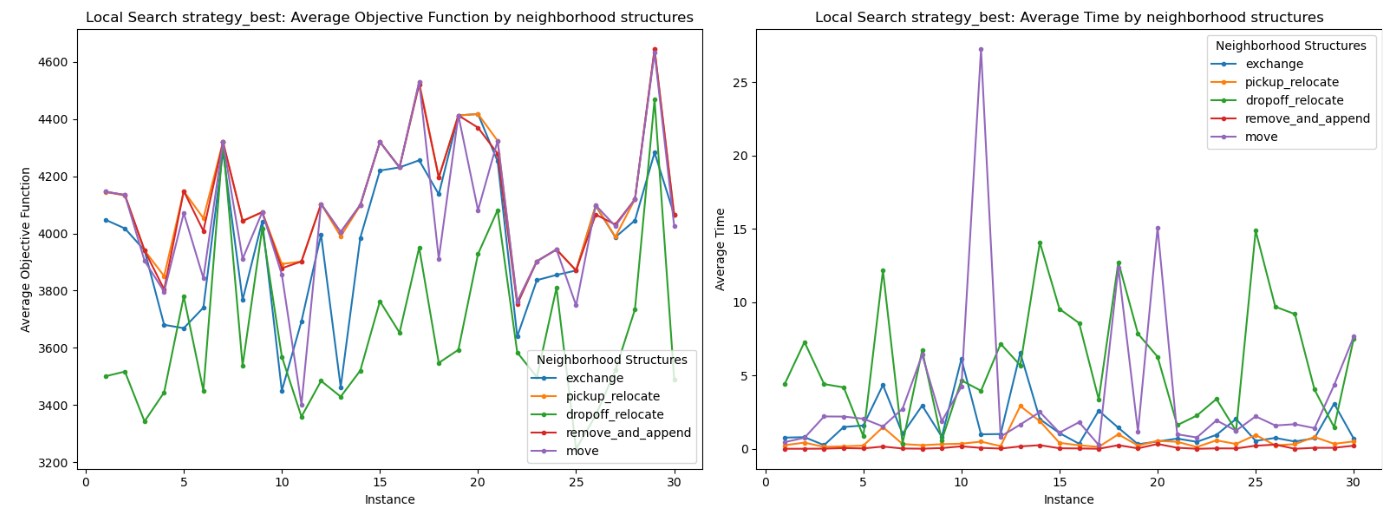
\includegraphics[width=\linewidth]{graphics/comparison_ns_ls.png}
    \caption{Comparison Neighborhood Structures: Comparison of average Objective Function and Run Time for 100 customers}
    \label{fig:comparison_ns_ls}
\end{figure}

\begin{figure}[H]
    \centering
    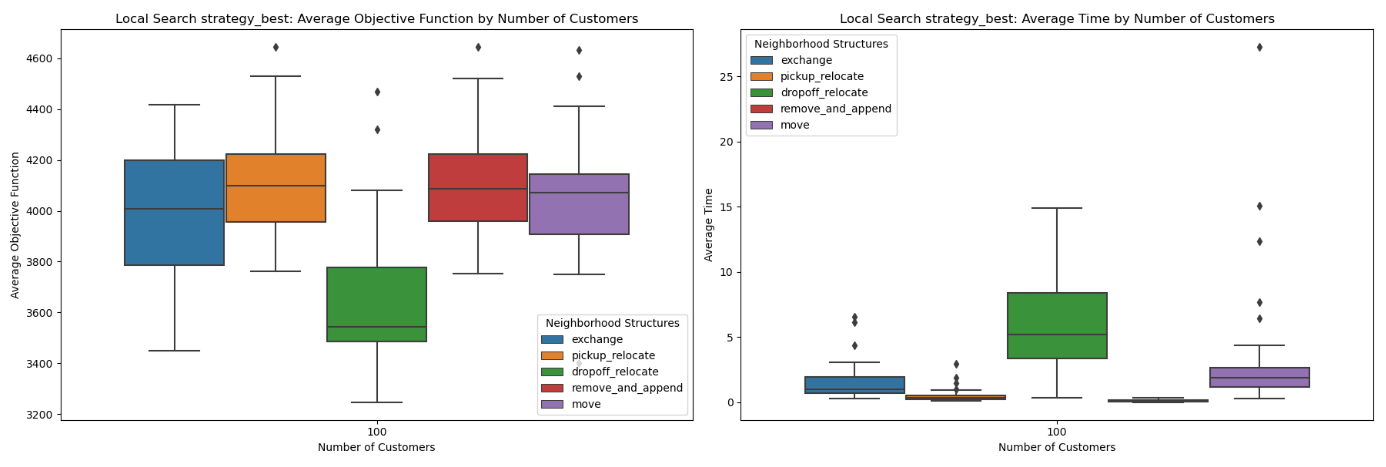
\includegraphics[width=\linewidth]{graphics/comparison_ns_ls_1.png}
    \caption{Comparison Neighborhood Structures: Comparison of average Objective Function and Run Time for 100 customers Boxplots}
    \label{fig:comparison_ns_ls_1}
\end{figure}

\subsubsection{Comparison of Step functions for Neighborhood structure dropoff relocate}

In this chapter, the two step functions best improvement and first improvement are compared to each other. Since the graphs look similar, we decided to only include the graphs for the neighborhood structure with the best results, which is the dropoff relocate neighborhood.

When comparing the first improvement strategy with the best improvement strategy, then one can see in Figure~\ref{fig:comparison_step_function_ls} and Figure~\ref{fig:comparison_step_function_ls_1} that the first improvement strategy leads in most cases to equal or better solutions, while being also much slower in runtime. These results might seem to be counterintuitive at first, but at least the reason for the increased runtime is very clear. Since the first improvement is chosen instead of the best possible, typically smaller steps towards a local optimum are made. This leads to more iterations that are necessary, until a local optimum is reached. For the solution quality our guess is that first improvement manages to prevent getting stuck too early in contrast to best improvement, who chooses the next move greedily.  

\begin{figure}[H]
    \centering
    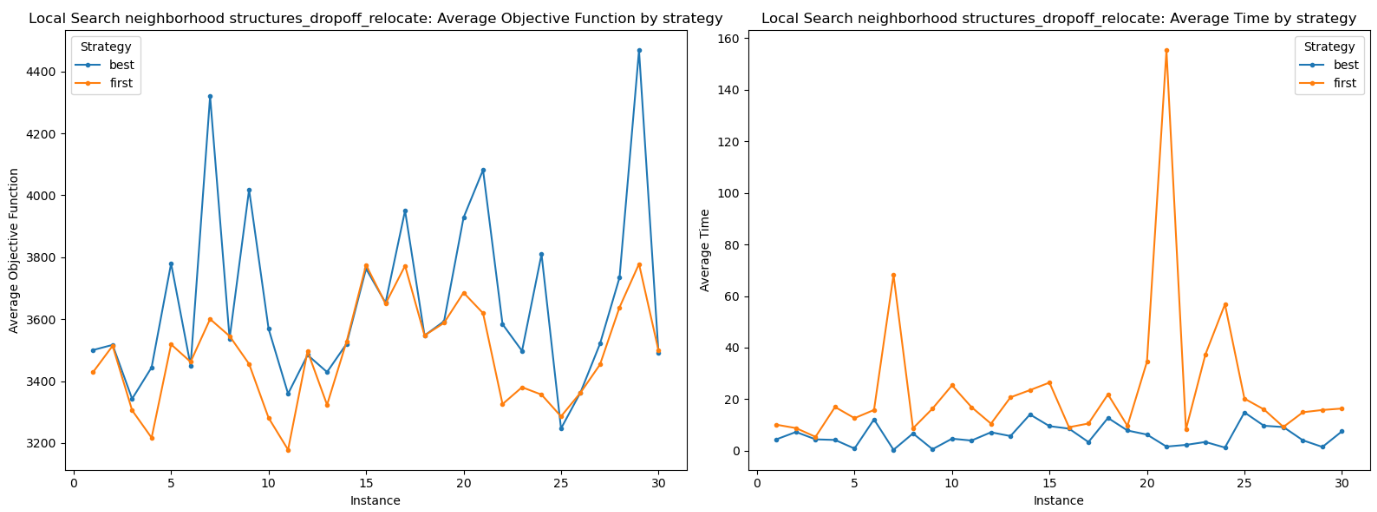
\includegraphics[width=\linewidth]{graphics/comparison_step_function_ls.png}
    \caption{Comparison Step Functions: Comparison of average Objective Function and Run Time for 100 customers}
    \label{fig:comparison_step_function_ls}
\end{figure}

\begin{figure}[H]
    \centering
    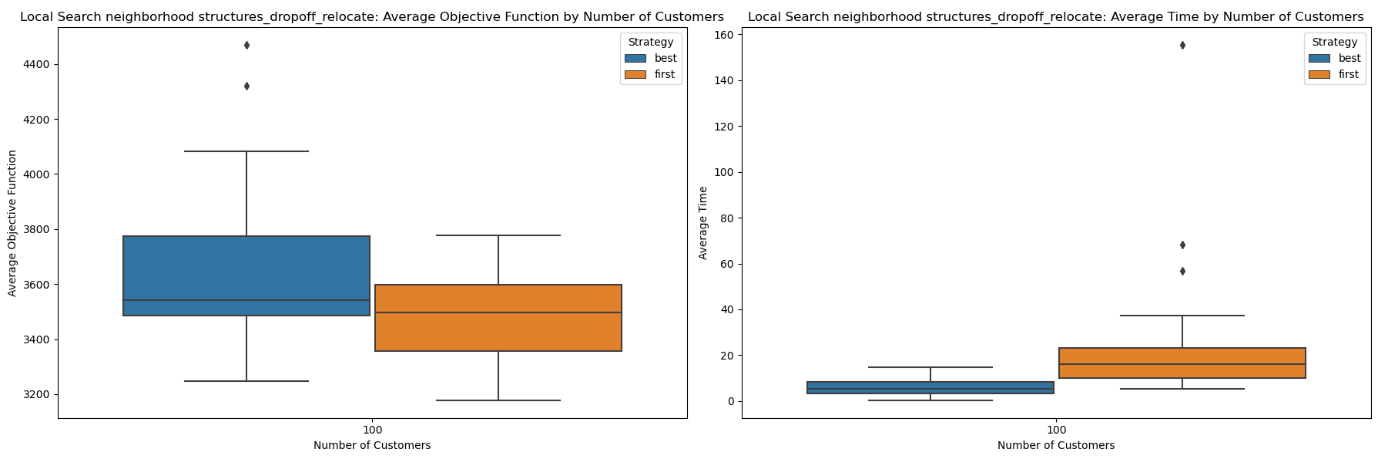
\includegraphics[width=\linewidth]{graphics/comparison_step_function_ls_1.png}
    \caption{Comparison Step Functions: Comparison of average Objective Function and Run Time for 100 customers Boxplots}
    \label{fig:comparison_step_function_ls_1}
\end{figure}


\subsection{Variable Neighborhood Descent}

In contrast to the local search, the algorithm for the variable neighborhood descent takes a list of neighborhood structures as an input. The default list is ["\emph{pickup$\_$relocate}", "\emph{dropoff$\_$relocate}", "\emph{exchange}", "\emph{move}"]. The idea behind the choice of this sequence is the following: Pickup relocate and dropoff relocate are improving the structure inside a vehicle and are simple to compute. The exchange neighborhood also does this to some extent, but also realizes an exchange between different vehicles, which would than again be improved by the relocate neighborhoods. Since these neighborhoods alone do not improve a solution, where one vehicle contains all customer request points and other vehicle paths are empty, the move neighborhood will be the one removing this kind of imbalance.

The implementation of variable neighborhood descent does not contain any problem specific modifications. Again, I refer to the neighborhood structures defined in Section~\ref{neighborhood}.

\subsubsection{Comparison of Step Functions}

As it was with the local search, the variable neighborhood descent also performs better when using first improvement. However, the running times are much faster and more stable for best improvement.

\begin{figure}[H]
    \centering
    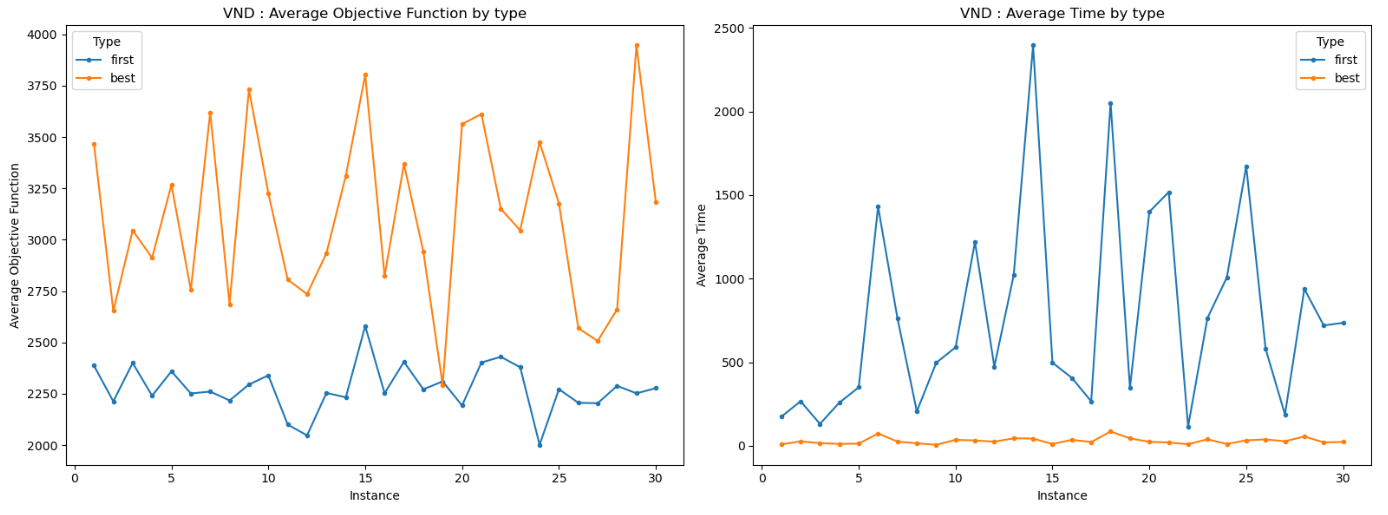
\includegraphics[width=\linewidth]{graphics/comparison_step_function_vdn.png}
    \caption{Comparison Step Functions: Comparison of average Objective Function and Run Time for 100 customers}
    \label{fig:comparison_step_function_vdn}
\end{figure}

\subsection{Greedy Randomized Adaptive Search Procedure}

The greedy randomized adaptive search procedure uses the randomized construction heuristic internally and has a fixed number of iterations without improvement as the stopping criteria. For improving on the received solution from the construction this algorithm uses variable neighborhood descent with its chosen default values.

\subsection{Simulated Annealing}

\pagebreak


\section{Experimental Results}

For the comparison of all algorithms we chose the best configuration for each algorithm. As presented in the previous chapters, these are: construction und randomized construction with reordering, the first improvement strategy for local search and variable neighborhood descent and the dropoff relocate neighborhood for local search.



\begin{figure}[H]
    \centering
    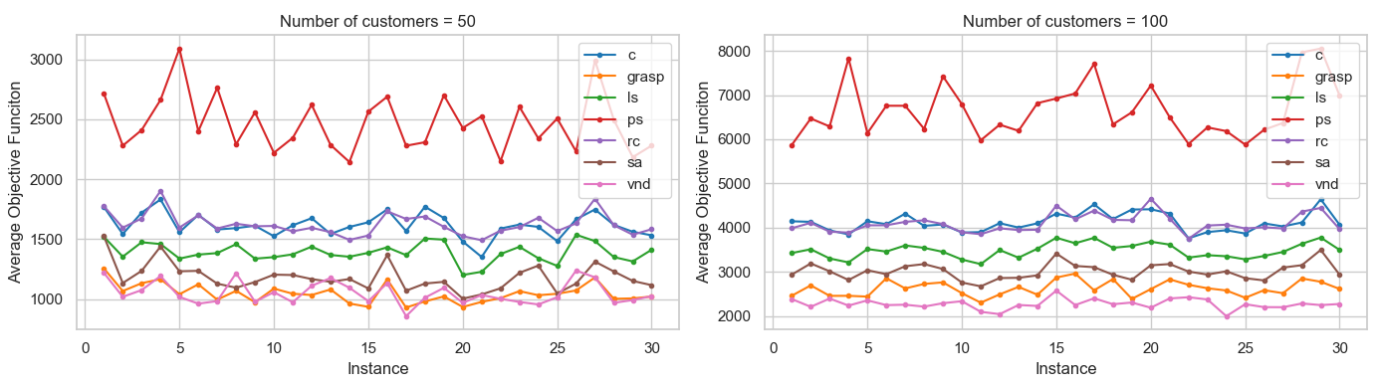
\includegraphics[width=\linewidth]{graphics/all_algorithms.png}
    \caption{Comparison The Solution Quality Of All Algorithms}
    \label{fig:all_algorithms}
\end{figure}

\begin{figure}[H]
    \centering
    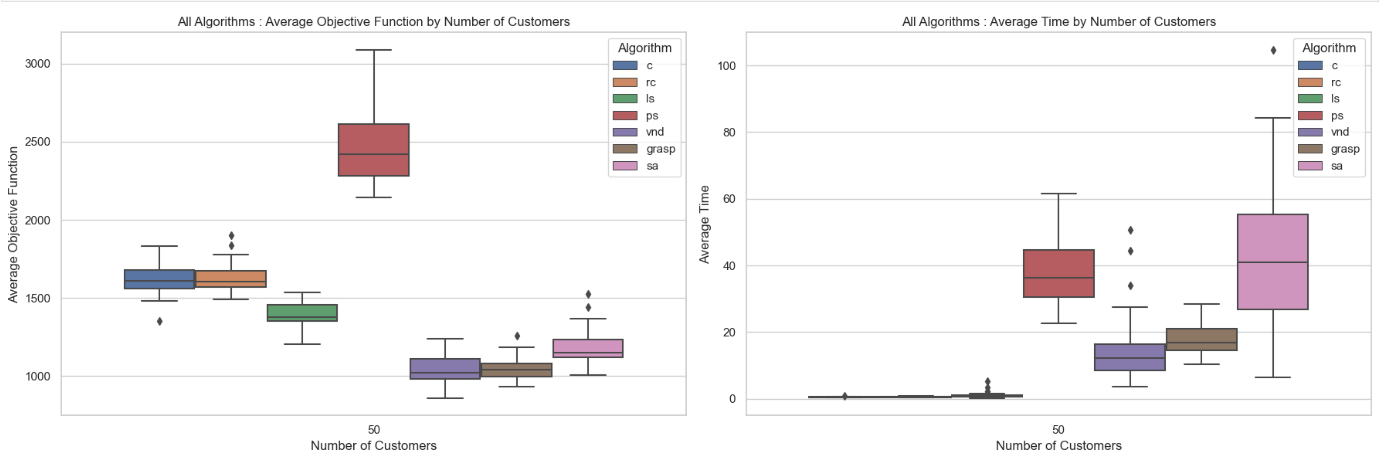
\includegraphics[width=\linewidth]{graphics/all_algorithms_1_50.png}
    \caption{Comparison The Solution Quality Of All Algorithms Boxplots for 50 customers}
    \label{fig:all_algorithms_1_50}
\end{figure}

\begin{figure}[H]
    \centering
    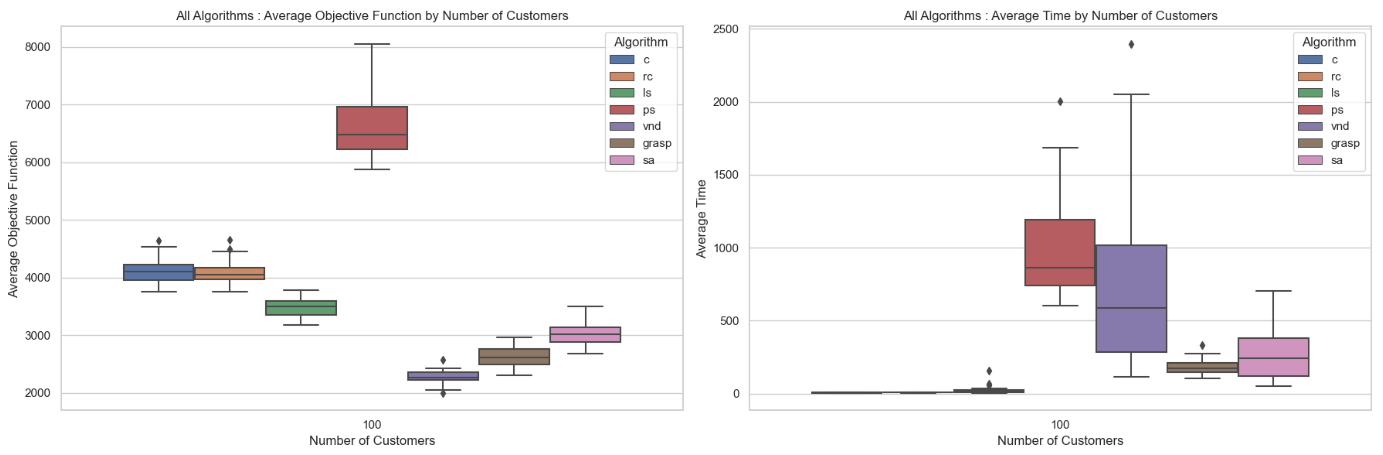
\includegraphics[width=\linewidth]{graphics/all_algorithms_1_100.png}
    \caption{Comparison The Solution Quality Of All Algorithms Boxplots for 100 customers}
    \label{fig:all_algorithms_1_100}
\end{figure}

\end{document}